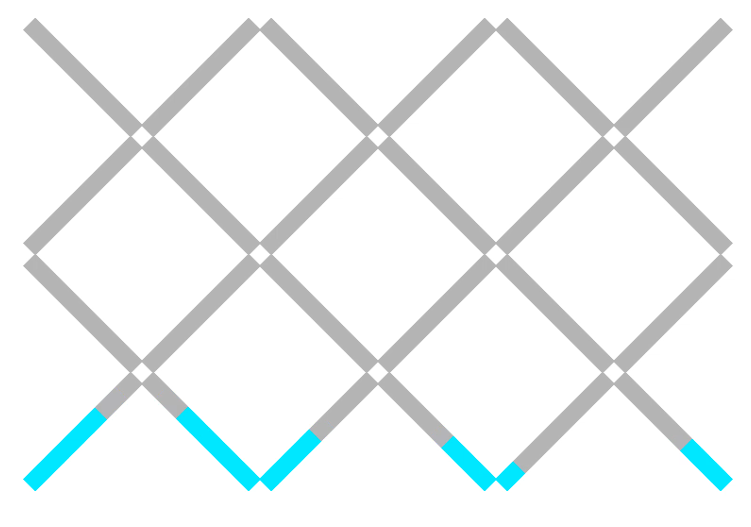
\includegraphics[height=6cm]{diagram/fig_initial-fill-distribution}
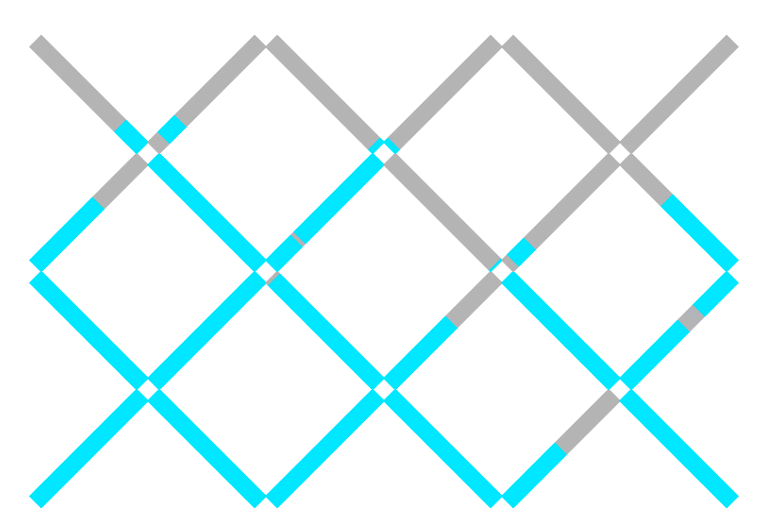
\includegraphics[height=6cm]{diagram/fig_final-fill-distribution}

Our model is initially set up such that the wetting fluid is low in saturation and is confined to the bottom of our network. A higher pressure is fixed for all nodes at the bottom layer, while a  low pressure is fixed for the top row. In all nodes, law of conservation of volume is applied, since mass is conserved and the phases are non-compressible. However for the bottom layer of nodes, the wetting fluid is injected as much required according to the sum of flow rates determined in the tubes connected to those nodes, while from the top layer of nodes a fluid is removed.

